\hypersetup{linkcolor=blue}
\chapter{Who Connects Better - M-Lab or Netflix?}\label{chapter:6}

We wanted to compare the Speedtest results to M-Lab media servers and to the Netflix OCA servers. As already discussed in \hyperref{section:relatedwork}, Netflix i.e. \textit{Fast.com} measures the the speedtest (bytes\_sec) it takes to download
25 MB of video file \cite{netflixfast}, whereas M-Lab tries to send as much data possible within 10 seconds (both upload and download) to a M-lab server \cite{mlabfaq}. Here, we will
be comparing the M-lab and Netflix achieved speedtest to get a clear picture about who gives better performance.
We will first compare the absolute values for both Netflix and M-Lab, individually over IPv4 and IPv6. Then, we will compare the Deltas for example, difference between M-Lab IPv4 measurement
and Netflix IPv4 measurement. Lets say, speedtest over IPv4 for M-Lab is tp(y) and speedtest over IPv4 for Netflix is tp(x), then the \textit{delta} will be $\Delta$tp = tp(y) - tp(x). Also, to note here that the
M-lab IPv6 test ran only till July 2017. 

\subsection*{Absolute}

\begin{figure}[!ht]
	\centering
	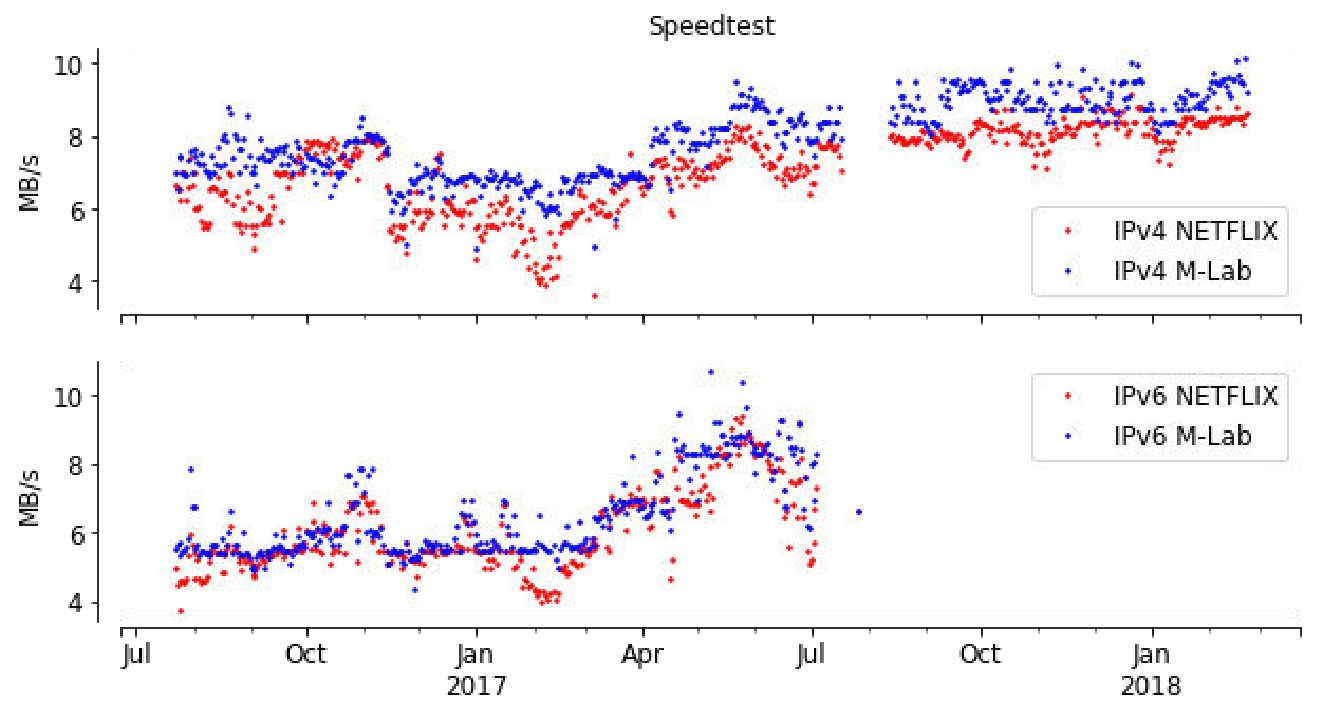
\includegraphics[keepaspectratio, height=5cm, width=15cm]{figures/mlab/netflix-throughput-timeseries-speedtest-netflix-separate.pdf}
	\caption[Speedtest Timeseries for M-Lab and Netflix Absolute]{Time series of Speedtest for individual address family's i.e. IPv4 and IPv6, for M-Lab and Netflix. We are considering the \textit{bytes\_sec} field
	,and speedtest for M-Lab is greater over both address family's and median speedtest for M-Lab and Netflix lies between 4-10 MB/s for both the families.}
	\label{fig:Speedtest Timeseries Absolute}
\end{figure}

\begin{figure}[!ht]
	\centering
	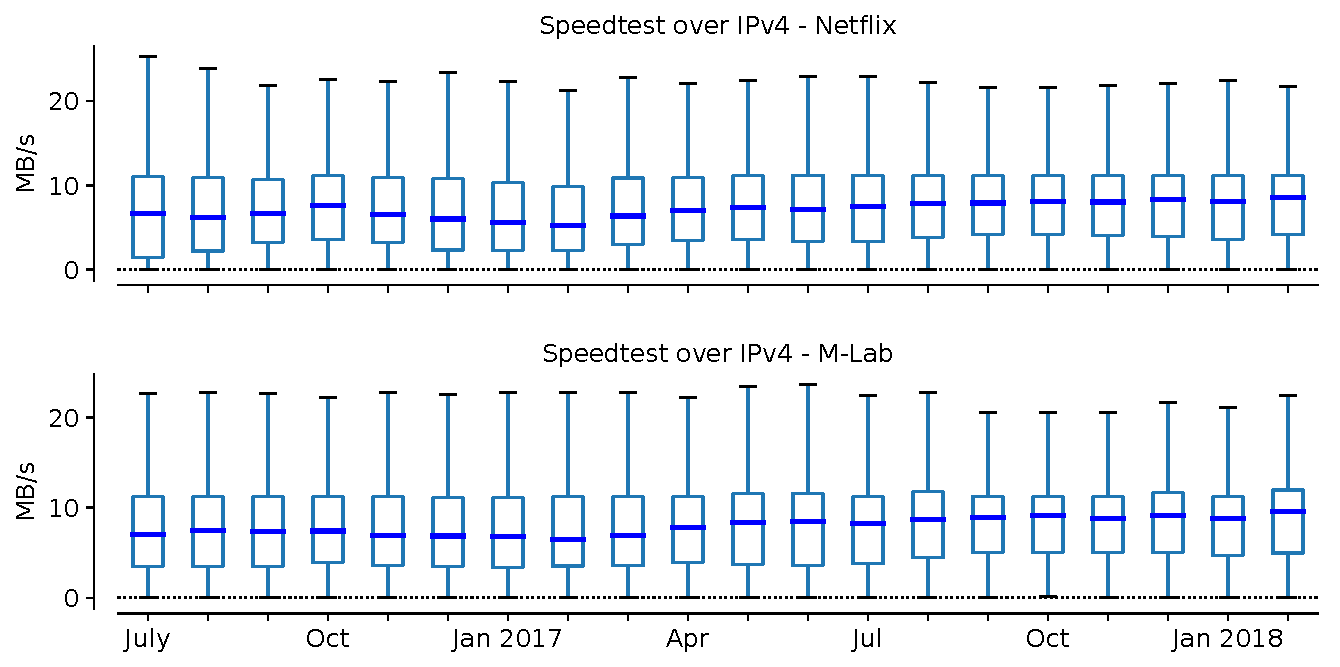
\includegraphics[keepaspectratio, height=4cm, width=15cm]{figures/mlab/netflix-throughput-boxplot-speedtest-separate-v4.pdf}
	\caption[Speedtest Boxplot Absolute IPv4]{Boxplot of speedtest over IPv4 for M-Lab and Netflix We can see the monthly variation here, also the median line resembles the time series in \cref{fig:Speedtest Timeseries Absolute}}
	\label{fig:Speedtest Boxplot Absolute IPv4}
\end{figure}

\begin{figure}[!ht]
	\centering
	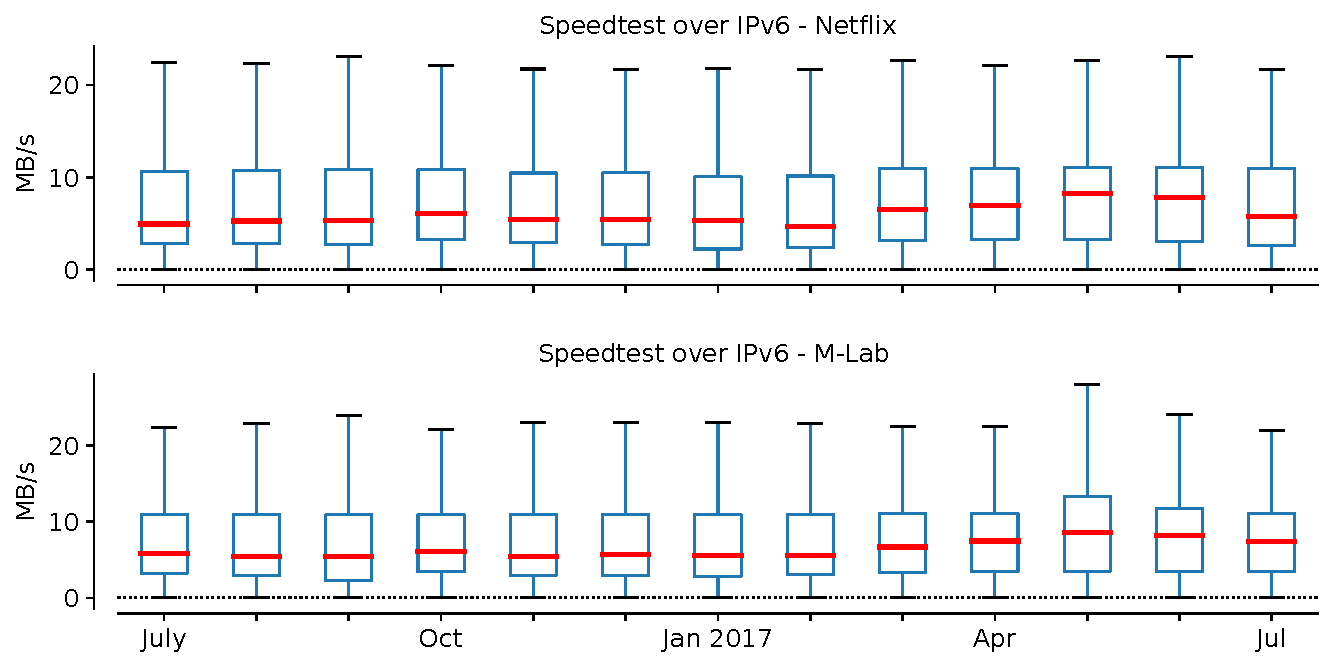
\includegraphics[keepaspectratio, height=4cm, width=15cm]{figures/mlab/netflix-throughput-boxplot-speedtest-separate-v6.pdf}
	\caption[Speedtest Boxplot Absolute IPv6]{Boxplot of speedtest over IPv6 for M-Lab and Netflix. We can see the monthly variation here, also the median line resembles the time series in \cref{fig:Speedtest Timeseries Absolute}}
	\label{fig:Speedtest Boxplot Absolute IPv6}
\end{figure}

We will first compare the timeseries plot for both M-Lab and Netflix, as can be seen in \cref{fig:Speedtest Timeseries Absolute} that the speedtest for M-Lab is greater over both address family's and median speedtest
for M-Lab and Netflix lies between 4-10 MB/s for both IPv4 and IPv6. Also, to note here that the speedtest is increasing over time for both M-lab and Netflix over boht IPv4 and IPv6.
We are considering the \textit{bytes\_sec} field, and we are taking the median aggregate across all probes on each day. To get more deeper insights
we also did the boxplot for IPv4 and IPv6 speedtest to compare M-Lab and Netflix performance, and as can be seen in \cref{fig:Speedtest Boxplot Absolute IPv4} and \cref{fig:Speedtest Boxplot Absolute IPv6} 
the monthly speedtest variation over IPv4 and IPv6. The median line resembles the time series in \cref{fig:Speedtest Timeseries Absolute}. We have 
converted the \textit{bytes\_sec} field into MB/s to get a more realistic view. \cref{fig:Speedtest CDF Absolute} shows the CDF of
speedtest over IPv4 and IPv6 for M-Lab and Netflix. We followed the same steps here,
and plotted the CDF of \textit{bytes\_sec} field. The CDF for individual address family's shows similar curves and does not give a clear difference
in the performance of M-Lab and Netflix over IPv4 and IPv6. 
We need to look into the deltas to get a more detailed performance comparison between M-Lab and Netflix.

\begin{figure}[!ht]
	\centering
	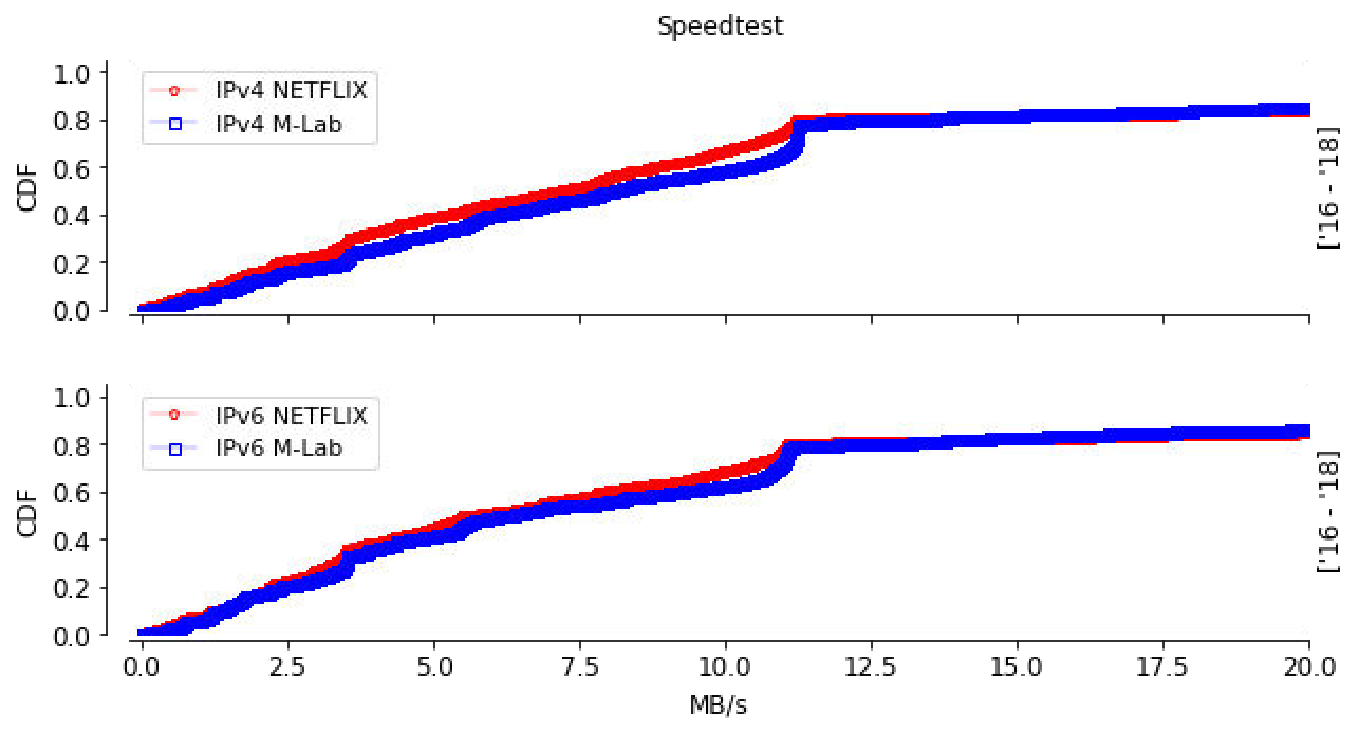
\includegraphics[keepaspectratio, height=5cm, width=15cm]{figures/mlab/netflix-throughput-difference-speedtest-separate.pdf}
	\caption[Speedtest CDF Absolute]{CDF of speedtest over IPv4 and IPv6 for M-Lab and Netflix, shows the similar curves over both the family's. We cannot see much difference in the performance of M-Lab and Netflix here.}
	\label{fig:Speedtest CDF Absolute}
\end{figure}

\FloatBarrier

\subsection*{Deltas}

\begin{figure}[!ht]
	\centering
	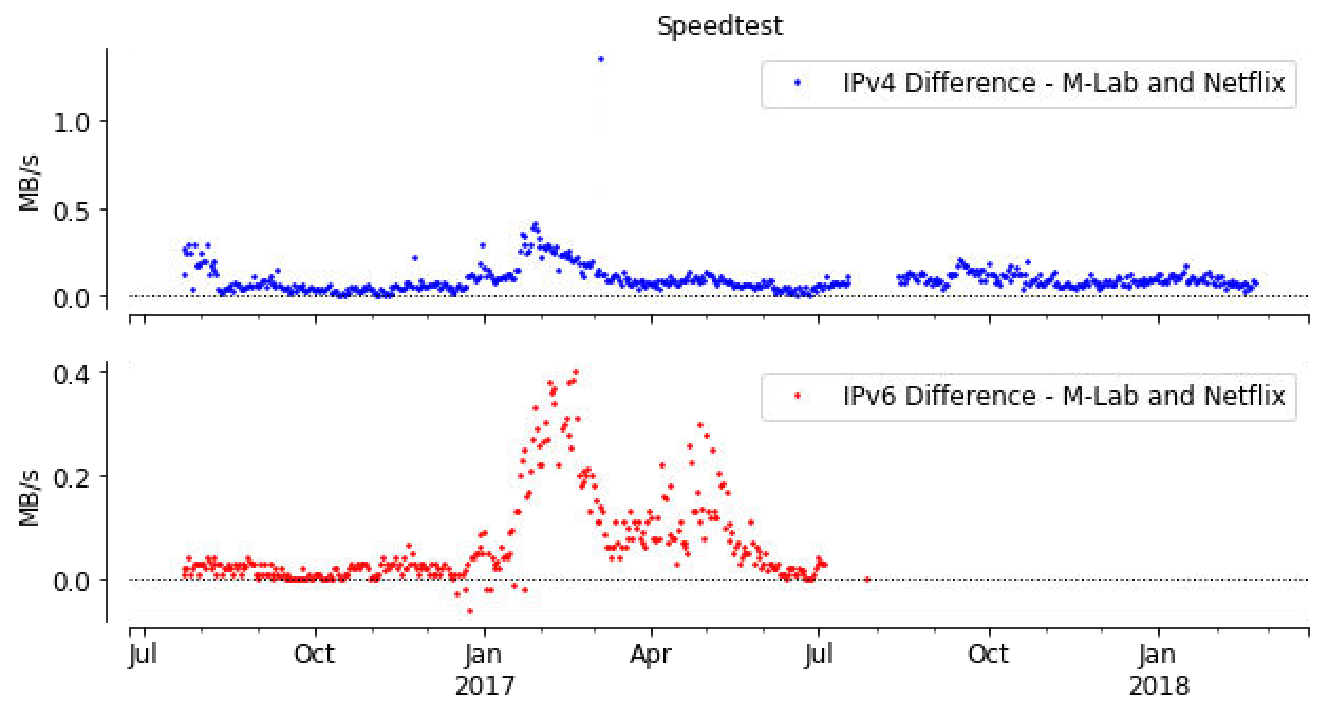
\includegraphics[keepaspectratio, height=5cm, width=15cm]{figures/mlab/netflix-throughput-timeseries-speedtest-netflix-difference.pdf}
	\caption[Speedtest Timeseries Delta]{Time series of difference of speedtest over IPv4 and IPv6 for M-Lab and Netflix. Here, The Netflix speedtest is subtracted from M-Lab speedtest. We plot the median aggregate across all probes on each day. The positive value indicates that
	the achieved speedtest is consistently lower for Netflix over both the Address family's.}
	\label{fig:Speedtest Timeseries Delta}
\end{figure}

\begin{figure}[!ht]
	\centering
	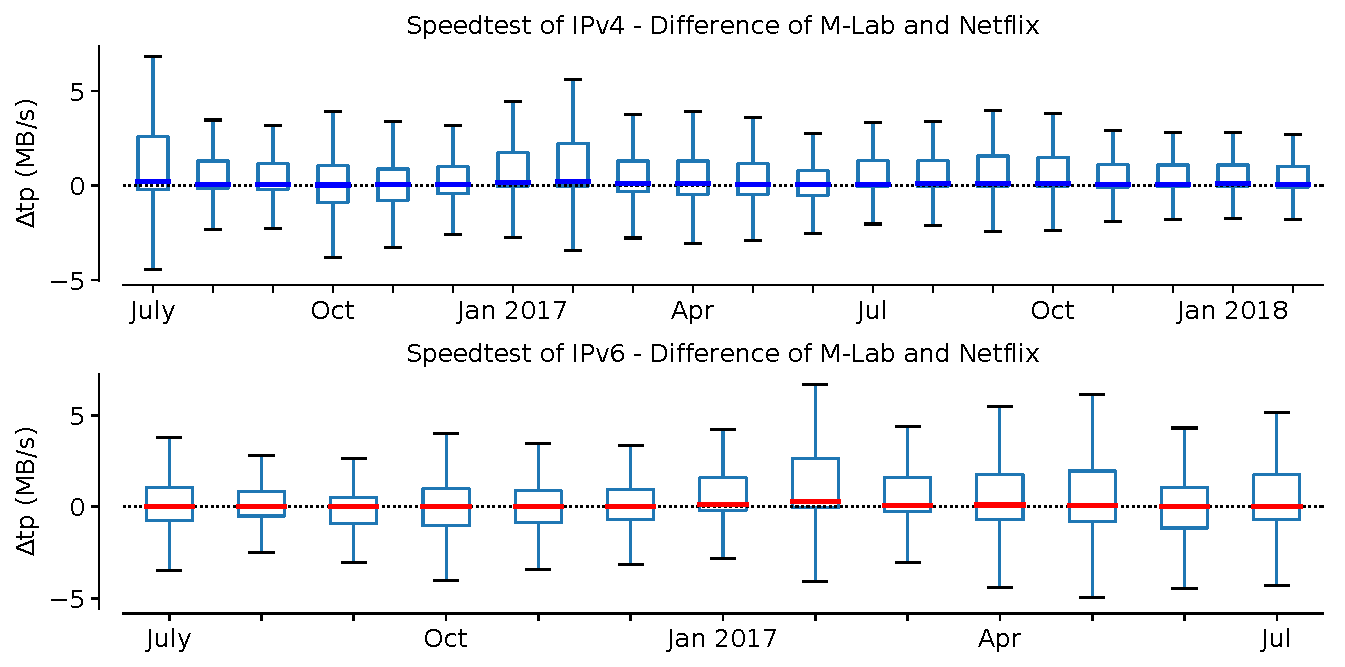
\includegraphics[keepaspectratio, height=5cm, width=15cm]{figures/mlab/netflix-throughput-boxplot-speedtest-difference.pdf}
	\caption[Speedtest Boxplot Delta]{Boxplot of difference of Speedtest for M-Lab and Netflix over IPv4 and IPv6. The figure also shows similar results as the time series \cref{fig:Speedtest Timeseries Delta}, depicting lower speedtest for Netflix over both IPv4 and IPv6.}
	\label{fig:Speedtest Boxplot Delta}
\end{figure}

We have already defined the terminology we are using here in the beginning of this chapter. We will use the equation that we defined above where $\Delta$tp is the difference in achieved speedtest
over the individual address family for M-Lab and Netflix. Also to note here, we are doing M-Lab minus Netflix here, so if the speedtest is positive then it means that the speedtest for M-Lab is better.
To plot the deltas, we first start with the time series, and \cref{fig:Speedtest Timeseries Delta} shows us the time series of median aggregate of speedtest across all probes over each day.
We can see that the difference is consistent over time and is lower for Netflix for both IPv4 and IPv6 over the whole duration. The positive value indicates a higher speedtest for M-Lab, also the difference lies between 0-0.5 MB/s for both the address families.
\cref{fig:Speedtest Boxplot Delta} shows the boxplot of difference of speedtest over IPv4 and IPv6. The median line shows similar curves as the time series \cref{fig:Speedtest Timeseries Delta}, depicting lower speedtest for Netflix.
To get a more clear picture about the performance, we plot the CDF of deltas of \textit{bytes\_sec} field. For CDF, we first compute the difference of speedtest for M-Lab and Netflix over IPv4 and IPv6 and then take the CDF of that difference.
Point to note here is that we are computing the difference between M-Lab and Netflix for a specific address family, i.e. difference between IPv4 measurement of M-Lab and Netflix and difference of IPv6 measurement
of M-Lab and Netflix.
\cref{fig:Speedtest CDF Delta} shows the CDF of difference of M-Lab and Netflix speedtest over IPv4 and IPv6. Around 59\% of the times, M-Lab achieved higher speedtest over Netflix for both the address families i.e. IPv4 and IPv6. We can see that according to these results M-Lab achieves higher speedtest over Netflix, Now,
one possible reason could be the Path length here, therefore in the next section we will consider the path length (TTL) for both M-Lab and Netflix to see how path length impact speedtest for these companies.

\begin{figure}[!ht]
	\centering
	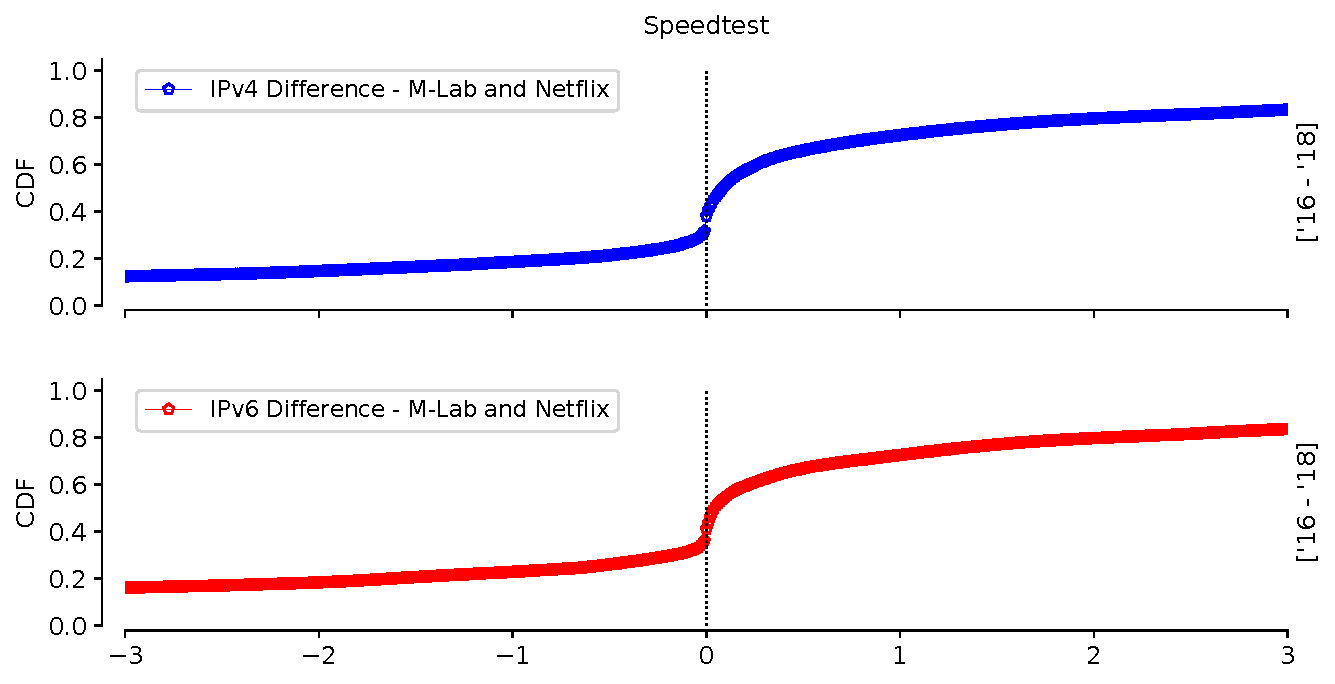
\includegraphics[keepaspectratio, height=5cm, width=15cm]{figures/mlab/netflix-throughput-difference-speedtest.pdf}
	\caption[Speedtest CDF delta]{CDF of Speedtest deltas for M-Lab and Netflix over Ipv4 and IPv6. Around 59\% of the times M-Lab achieved higher speed over Netflix for both the address family's.}
	\label{fig:Speedtest CDF Delta}
\end{figure}

\subsection*{Is shorter path length impacting the Speedtest for M-Lab?}

As already discussed in the previous section that speedtest to M-Lab servers are better as compared to speedtest to Netflix OCA servers. We wanted to find the reason for this and therefore,
we would like to compare the path length i.e. TTL to M-Lab and Netflix servers. We therefore, here are comparing the TTL over IPv4 and IPv6 for M-Lab and Netflix. Also to note here, we are analysing the TTL
for each probe. The reason ffor doing is that TTL as a factor is dependent on location and network of the probe. So for some probe the TTL to M-Lab could be less and for some it could be more.
We will thus see the distribution of Speedtest and TTL for each probe. As there are around 100 probes and we can't display everything in this study, we are just showing the results from one probe (Number 33).
The results from this probe is trated as an example and mimic the results from most of the probes. The rest fo the graphs from each probe can be found at /data/akapoor/.

 \begin{figure}[!ht]
	\centering
	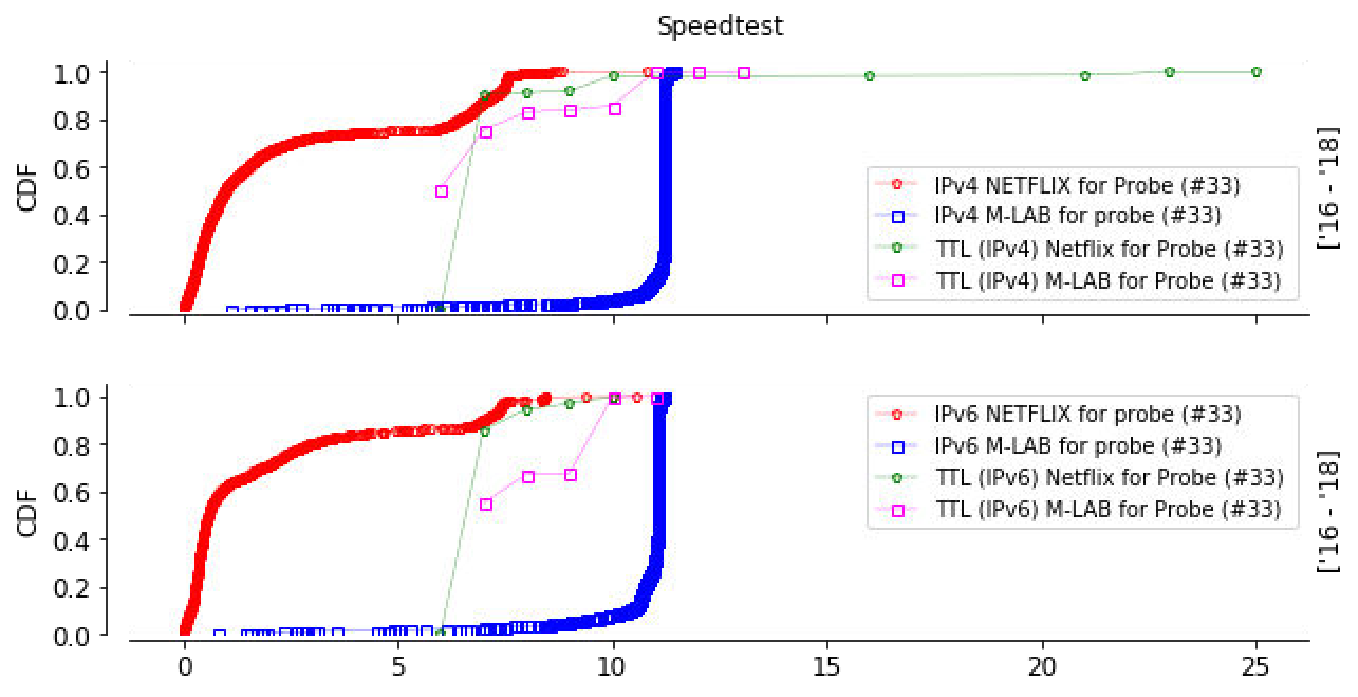
\includegraphics[keepaspectratio, height=5cm, width=15cm]{figures/mlab/ttl-speedtest-cdf-probe-separate-probe-33.pdf}
	\caption[Speedtest CDF Absolute for Probe 33]{CDF of speedtest and TTL over IPv4 and IPv6 for M-Lab and Netflix for Probe number 33. As can be seen, the speedtest for M-Lab is more but the TTL is also less as compared to Netflix.}
	\label{fig:Speedtest CDF Absolute for Probe 33}
\end{figure}

\begin{figure}[!ht]
	\centering
	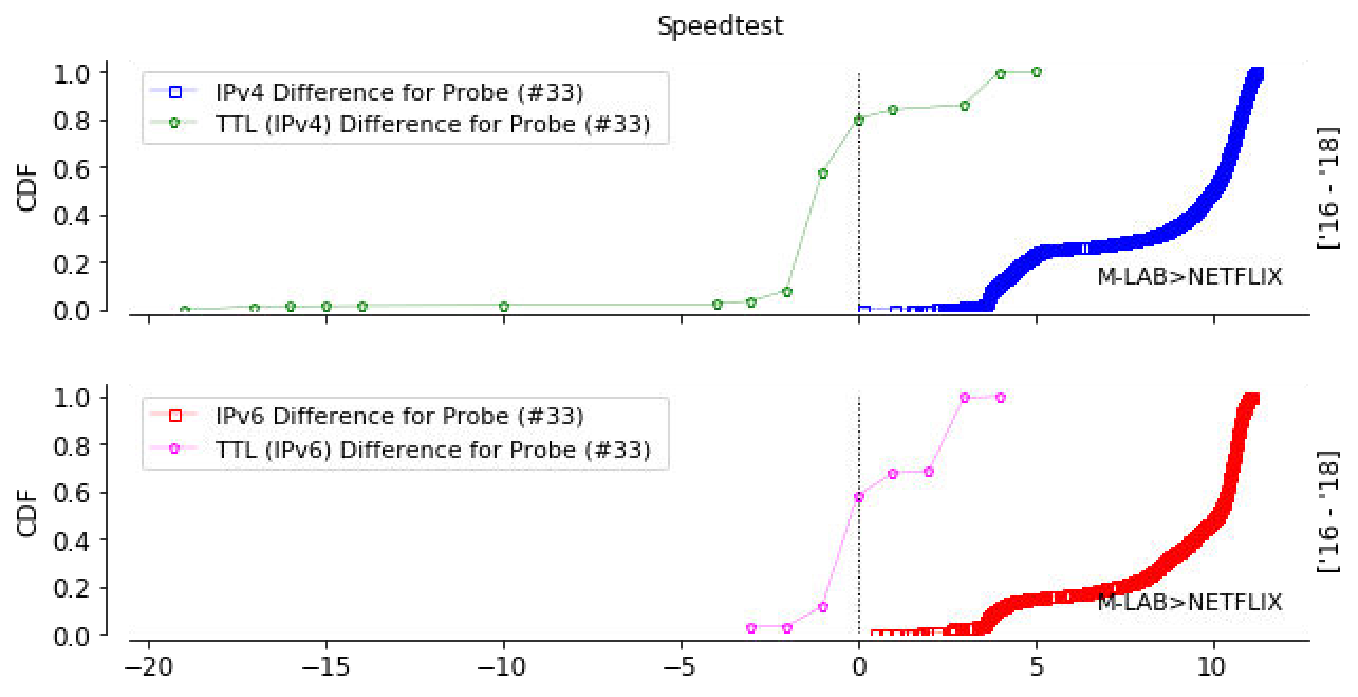
\includegraphics[keepaspectratio, height=5cm, width=15cm]{figures/mlab/ttl-speedtest-cdf-probe-33.pdf}
	\caption[Speedtest CDF delta for Probe 33]{CDF of Speedtest and TTL deltas for M-Lab and Netflix over IPv4 and IPv6 for probe number 33. As can be seen from the graph, the speedtest for M-Lab is better than speedtest for Netflix
but the TTL for M-Lab is shorter i.e. less path length as compared to TTL for Netflix.}
	\label{fig:Speedtest CDF Delta for Probe 33}
\end{figure}

Here, \cref{fig:Speedtest CDF Absolute for Probe 33} shows us the CDF of speedtest and TTL over IPv4 and IPv6 for M-Lab and Netflix for probe number 33. As can be seen, the speedtest for M-Lab is more but the TTL is also less as compared to Netflix. This shows us
that path length impact speedtest. To be more sure, we will now consider the deltas here, and as can be seen in \cref{fig:Speedtest CDF Delta for Probe 33} the speedtest for M-Lab is better than speedtest for Netflix
but the TTL for M-Lab is shorter i.e. less path length as compared to TTL for Netflix. The TTL curve on the left side of Zero axis suggest that the TTL is shorter for M-Lab as we are taking the difference of M-lab minus Netflix here.
Therefore, we can conclude that, path length impacts speedtest/throughput for M-Lab and Netflix.